
%%%%%%%%%%%%%%%%%%%%%%%%%%%%%%%%%%%%%%%%%%%%%%%%%%%%%%%%%%%%%%%%%%%%%%%%%%%%%%%%%%%%%%%
%%%%%%%%%%%%%%%%%%%%%%%%%%%%%%%%%%%%%%%%%%%%%%%%%%%%%%%%%%%%%%%%%%%%%%%%%%%%%%%%%%%%%%%
% 
% This top part of the document is called the 'preamble'.  Modify it with caution!
%
% The real document starts below where it says 'The main document starts here'.

\documentclass[12pt]{article}

\usepackage{amssymb,amsmath,amsthm}
\usepackage[top=1in, bottom=1in, left=1.25in, right=1.25in]{geometry}
\usepackage{fancyhdr}
\usepackage{enumerate}
\usepackage{listings}
\usepackage{graphicx}
\usepackage{float}

\usepackage{mwe}
\usepackage{caption}
\usepackage{subcaption}
% Comment the following line to use TeX's default font of Computer Modern.
\usepackage{times,txfonts}



\makeatletter
\renewcommand*\env@matrix[1][*\c@MaxMatrixCols c]{%
  \hskip -\arraycolsep
  \let\@ifnextchar\new@ifnextchar
  \array{#1}}
\makeatother

\newtheoremstyle{homework}% name of the style to be used
  {18pt}% measure of space to leave above the theorem. E.g.: 3pt
  {12pt}% measure of space to leave below the theorem. E.g.: 3pt
  {}% name of font to use in the body of the theorem
  {}% measure of space to indent
  {\bfseries}% name of head font
  {:}% punctuation between head and body
  {2ex}% space after theorem head; " " = normal interword space
  {}% Manually specify head
\theoremstyle{homework} 

% Set up an Exercise environment and a Solution label.
\newtheorem*{exercisecore}{Exercise \@currentlabel}
\newenvironment{exercise}[1]
{\def\@currentlabel{#1}\exercisecore}
{\endexercisecore}

\newcommand{\localhead}[1]{\par\smallskip\noindent\textbf{#1}\nobreak\\}%
\newcommand\solution{\localhead{Solution:}}

%%%%%%%%%%%%%%%%%%%%%%%%%%%%%%%%%%%%%%%%%%%%%%%%%%%%%%%%%%%%%%%%%%%%%%%%
%
% Stuff for getting the name/document date/title across the header
\makeatletter
\RequirePackage{fancyhdr}
\pagestyle{fancy}
\fancyfoot[C]{\ifnum \value{page} > 1\relax\thepage\fi}
\fancyhead[L]{\ifx\@doclabel\@empty\else\@doclabel\fi}
\fancyhead[C]{\ifx\@docdate\@empty\else\@docdate\fi}
\fancyhead[R]{\ifx\@docauthor\@empty\else\@docauthor\fi}
\headheight 15pt

\def\doclabel#1{\gdef\@doclabel{#1}}
\doclabel{Use {\tt\textbackslash doclabel\{MY LABEL\}}.}
\def\docdate#1{\gdef\@docdate{#1}}
\docdate{Use {\tt\textbackslash docdate\{MY DATE\}}.}
\def\docauthor#1{\gdef\@docauthor{#1}}
\docauthor{Use {\tt\textbackslash docauthor\{MY NAME\}}.}
\makeatother

% Shortcuts for blackboard bold number sets (reals, integers, etc.)
\newcommand{\Reals}{\ensuremath{\mathbb R}}
\newcommand{\Nats}{\ensuremath{\mathbb N}}
\newcommand{\Ints}{\ensuremath{\mathbb Z}}
\newcommand{\Rats}{\ensuremath{\mathbb Q}}
\newcommand{\Cplx}{\ensuremath{\mathbb C}}
%% Some equivalents that some people may prefer.
\let\RR\Reals
\let\NN\Nats
\let\II\Ints
\let\CC\Cplx

%%%%%%%%%%%%%%%%%%%%%%%%%%%%%%%%%%%%%%%%%%%%%%%%%%%%%%%%%%%%%%%%%%%%%%%%%%%%%%%%%%%%%%%
%%%%%%%%%%%%%%%%%%%%%%%%%%%%%%%%%%%%%%%%%%%%%%%%%%%%%%%%%%%%%%%%%%%%%%%%%%%%%%%%%%%%%%%
% 
% The main document start here.

% The following commands set up the material that appears in the header.
\doclabel{STAT 401: Homework 11}
\docauthor{Stefano Fochesatto}
\docdate{\today}


%\begin{figure}[H]
%  \begin{center}
%  \caption{}
%  \includegraphics[\textwidth]{}
%  \end{center}
%\end{figure}

% \textbf{Code:}
% \begin{center}
% \lstinputlisting{}
% \end{center} 



\begin{document}

\begin{exercise}{1} Refer to problem 8.5 for a short explanation of the BigMac2003 data set. Then do the following, 
  \begin{enumerate}
    \item Check the five diagnostics on model assumptions in the linear model that includes Bigmac as the response and 
    all nin predictors. Based on these diagnostics, which model assumption do not appear to be valid. \\
    \solution First we can check for non linearity in the model, plotting the residuals and performing Tukey's test we get the following, 
\begin{figure}[H]
  \begin{center}
  \caption{Residual Plot for Each Predictor}
  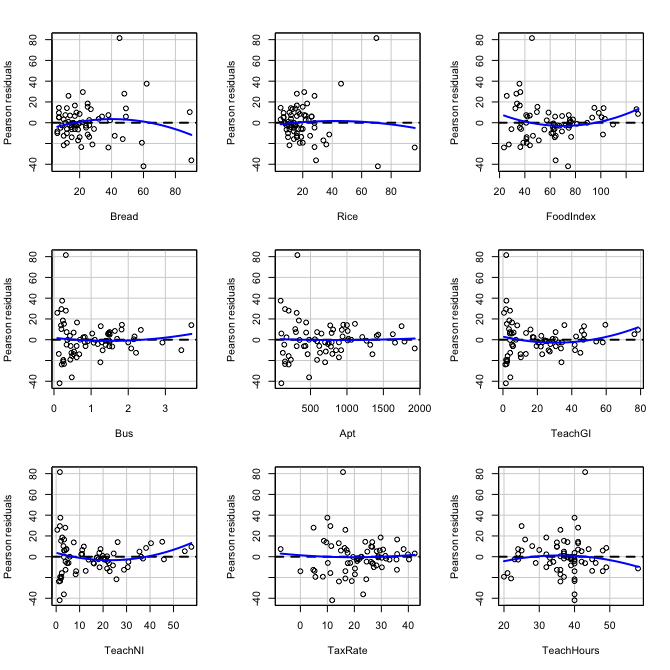
\includegraphics[width = \textwidth]{Rplot.png}
  \end{center}
\end{figure}
\begin{figure}[H]
  \begin{center}
  \caption{Residual Plot for Entire Model}
  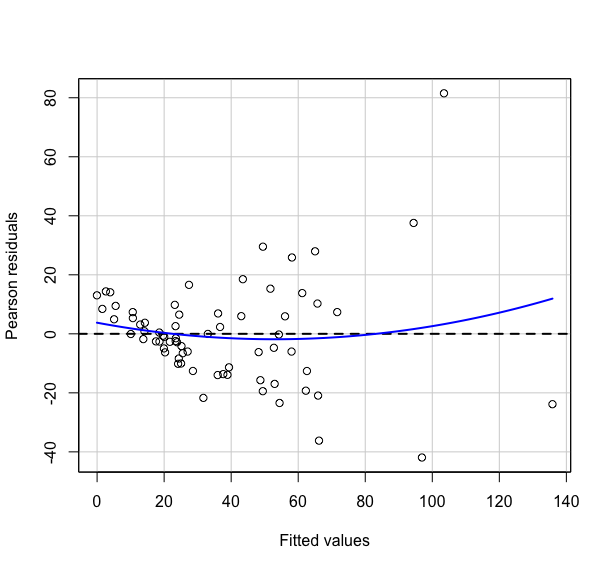
\includegraphics[width = \textwidth]{Rplot01.png}
  \end{center}
\end{figure}
      \textbf{Code:}
       \begin{center}
       \lstinputlisting{r1.txt}
       \end{center} 
       Generally the residual plot show a low degree of curvature in the fitted second order model. As suggested by the results of Tukey's test 
       I would say that this model achieves a high degree of linearity. \\ 
       Since we already have the residual plots it would be appropriate to test for non-constant variance. Looking at the fitted value
       residuals we can see a wedge pattern in the residuals, this suggests a very strong degree of non constant variance. We can also see this in almost all of 
       the predictors. Testing this with the Breusch-Pagan test we can see that, with a p-value on the order of $10^{16}$ we cannot assume constant variance in our error.\\
       \textbf{Code:}
       \begin{center}
       \lstinputlisting{r2.txt}
       \end{center} 
       
       
       
       Looking at the residual plot again it does seem possible there could be a couple of outliers, checking the residuals using the outlierTest() function we get, 
       that there is at least one outlier, which would warrant further analysis.\\
       \textbf{Code:}
       \begin{center}
       \lstinputlisting{r3.txt}
       \end{center} 
       In the same vein we can test for influence points using Cooks Distance. Using the $4/n$ criteria there are 5 influential places in the data set
       which we attained using cooks.distance() function, 
       \begin{figure}[H]
        \begin{center}
        \caption{Residual Plot Cooks Distance}
        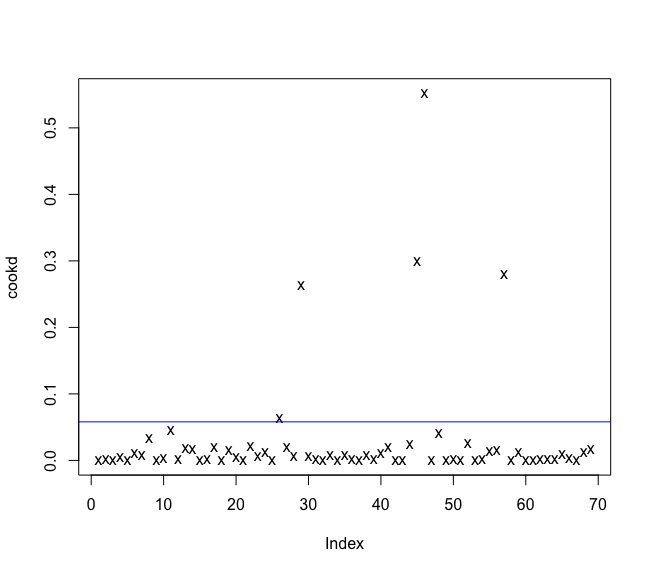
\includegraphics[width = \textwidth]{Rplot02.png}
        \end{center}
      \end{figure}
      \textbf{Code:}
      \begin{center}
      \lstinputlisting{r4.txt}
      \end{center} 


      Checking for autocorrelation in our residuals, we can use the Durbin-Watson test. Doing so we get a p-value of .98
      which means on the $\alpha = .05$ level our residuals do not show autocorrelation. \\
      \textbf{Code:}
      \begin{center}
      \lstinputlisting{r5.txt}
      \end{center} 

      Finally using the Shapiro-Wilk test we can test for normality among our residuals. Doing so we get a p-value on the 
      order of $10^{-5}$ so our residuals are not normally distributed.
      \textbf{Code:}
      \begin{center}
      \lstinputlisting{r6.txt}
      \end{center} 
      In general this model fails a majority of our diagnostics, specifically the model has several leverage points and outliers, demonstrates 
      non-constant variance, and non-normally distributed residuals. I would not trust the results of this model. 
      \newpage

      \item[b.] Find the Box-Cox tranformation for the response variable and make theneares ladder-of-powers transformation 
      to it. Recheck the five diagnostics with the transformed response. What is the transformation and which assumptions still appear to be 
      invalid?\\
      \solution We can find the nearest ladder-of-powers transformation using the powerTransformation() function. Doing so we get that the response should be 
      raised to the power of $-.5$. Performing the diagnostics again we get that the model now has constant variance in the residuals, normally distributed residuals, and smaller outliers. There 
      are still leverage points under the $4/n$ criteria, but the model is significantly more trustworthy. \\
      \textbf{Code:}
      \begin{center}
      \lstinputlisting{r7.txt}
      \end{center} 
      \begin{figure}[H]
        \begin{center}
        \caption{Residual Plot for Transformed Model}
        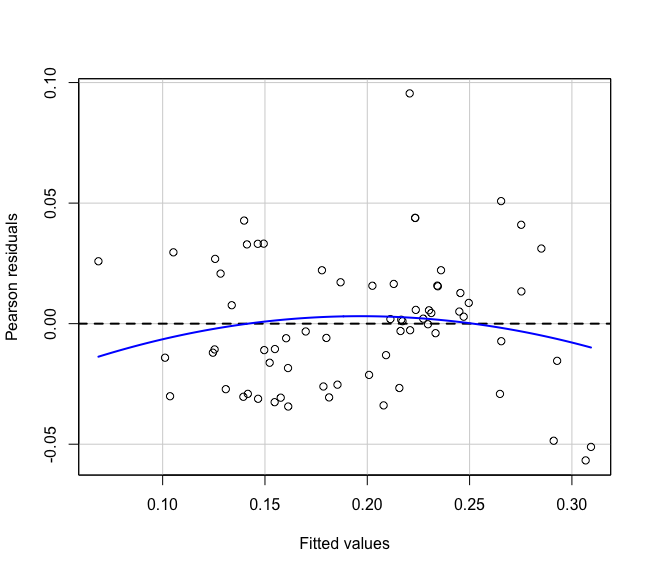
\includegraphics[width = \textwidth]{Rplot04.png}
        \end{center}
      \end{figure}
      \begin{figure}[H]
        \begin{center}
        \caption{Residual Plot Cooks Distance}
        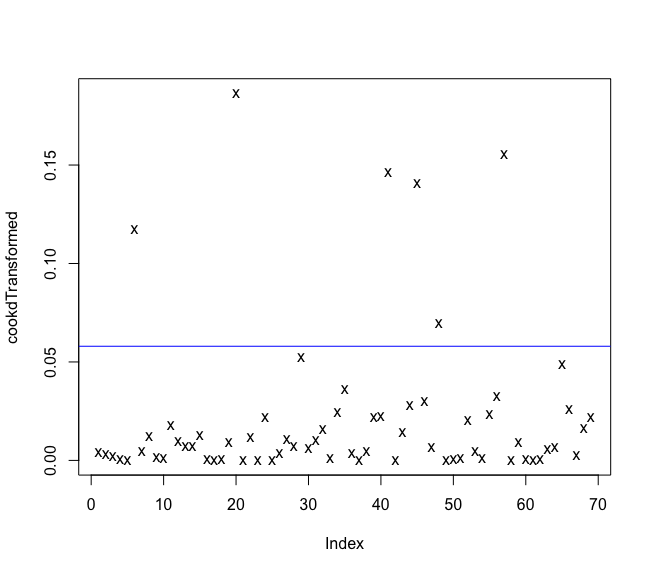
\includegraphics[width = \textwidth]{Rplot05.png}
        \end{center}
      \end{figure}




      \newpage

      \item[c.] Use the generalized Box-Cox tranformaiton for the predictors and find transformation from the 
      ladder of powers to make the transformed predictors as close to linearly related as possible. Recheck the five diagnostics. what is 
      the transformation for each of the nine predictors and which assumptions still appear to be invalid. \\
      \solution  First we need to do as the hint suggests and smear the data that this is less than or equal to zero to use the 
      powerTransform() function. Doing so we get that we should log transform Bread, Rice, FoodIndex, Bus, TeachGI and TeachNI. We should also 
      square root Apt and raise TaxRate to the 1.1 power. Running diagnostics on the fitted model, we see that it performs significantly worse than 
      when we just transformed the response. The model show significant non-linear, non-normal residuals with non-constant variance. It also shows multiple leverage points and 
      even greater outliers. The model does appear to show no autocorrelation. This model is not trustworthy.\\
      \textbf{Code:}
      \begin{center}
      \lstinputlisting{r8.txt}
      \end{center} 
      \begin{figure}[H]
        \begin{center}
        \caption{Residual Plot for Each Transformed Predictor}
        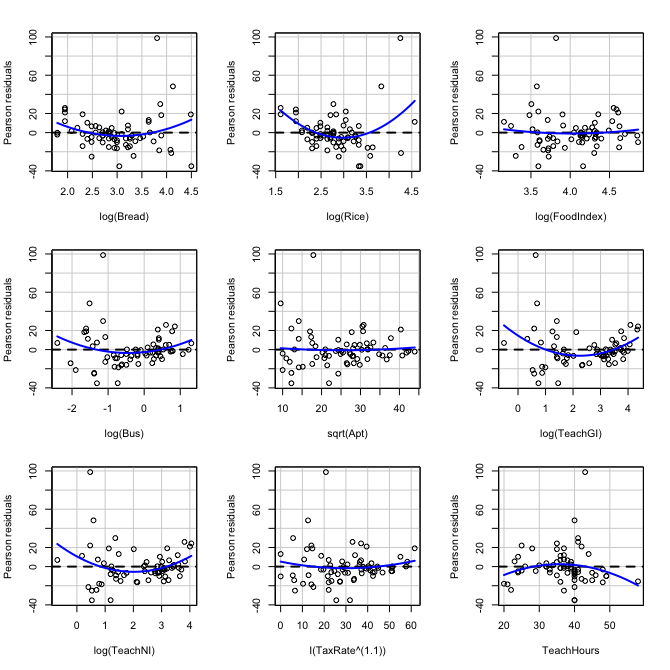
\includegraphics[width = \textwidth]{Rplot06.png}
        \end{center}
      \end{figure}
      \begin{figure}[H]
        \begin{center}
        \caption{Residual Plot for Transformed Predictor Model}
        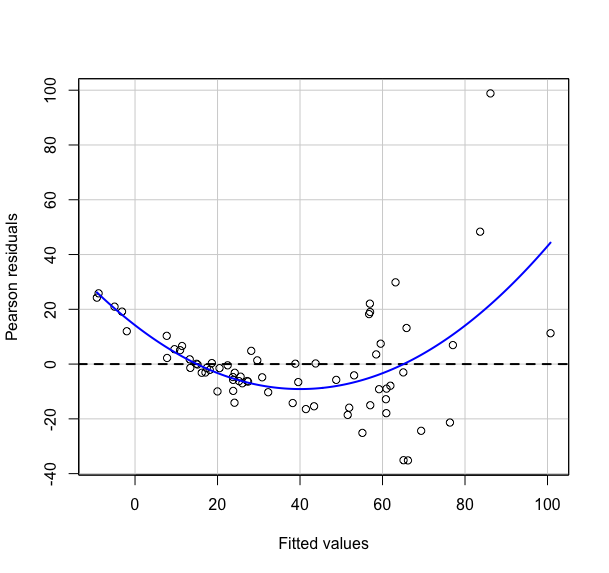
\includegraphics[width = \textwidth]{Rplot07.png}
        \end{center}
      \end{figure}
      \begin{figure}[H]
        \begin{center}
        \caption{Residual Plot Cooks Distance}
        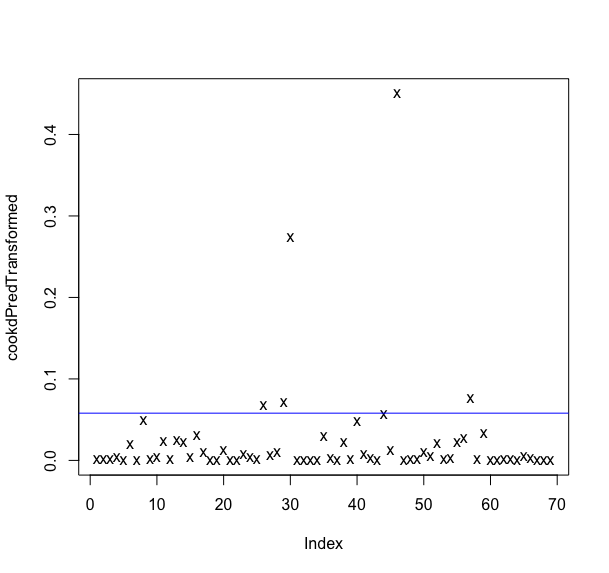
\includegraphics[width = \textwidth]{Rplot08.png}
        \end{center}
      \end{figure}
      \newpage


      \item[d.] Given the predictor transformation made in the last part, use the Box-Cox method to find a transformation of 
      BigMac. Recheck the five diagnostics. What is the transformation ans which assumptions still appear to be invalid. \\
      \solution Finally transforming both the predictor and response using the powerTransform() function we get that BigMac should 
      once again be raised to the power of $-.5$. Running the diagnostics to the fitted model we get passes all assumptions except that 
      its residuals are not normally distributed, and it still has multiple leverage points. \\
      \textbf{Code:}
      \begin{center}
      \lstinputlisting{r9.txt}
      \end{center} 
      \begin{figure}[H]
        \begin{center}
        \caption{Predictor Residual Plots for Full Transformed Model}
        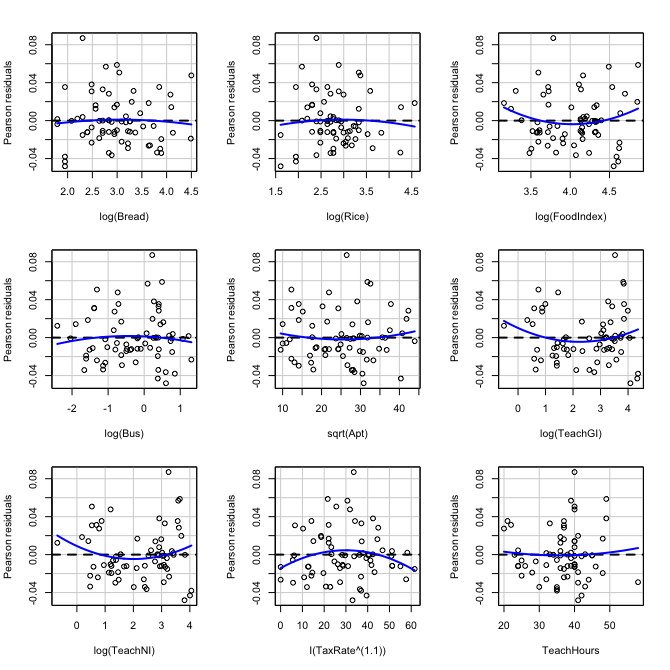
\includegraphics[width = \textwidth]{Rplot09.png}
        \end{center}
      \end{figure}
      \begin{figure}[H]
        \begin{center}
        \caption{Residual Plot for Full Transformed Model}
        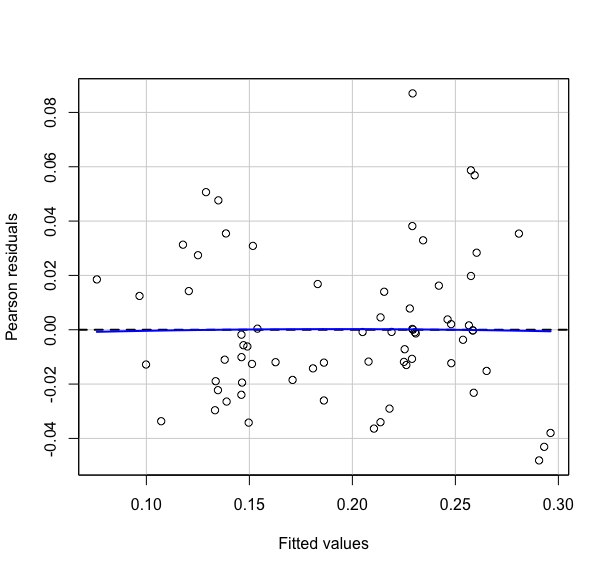
\includegraphics[width = \textwidth]{Rplot10.png}
        \end{center}
      \end{figure}
      \begin{figure}[H]
        \begin{center}
        \caption{Residual Plot Cooks Distance}
        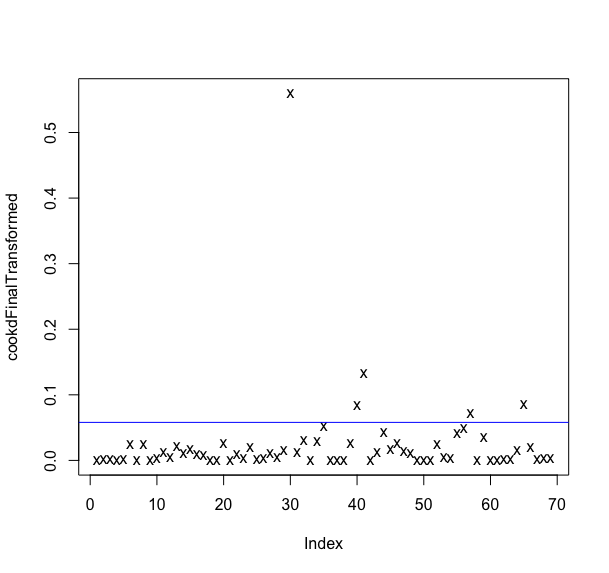
\includegraphics[width = \textwidth]{Rplot11.png}
        \end{center}
      \end{figure}
      \newpage

      \item[e]. Are you satisfied wiht the final model? Why or why not?\\
      \solution I am not satisfied with the final model. The final model does not produce normally distributed residuals, it would likely be 
      better to just use the first transformed model where we simply transformed the response variable.  
  \end{enumerate}
\end{exercise}
\newpage

\begin{exercise}{10.4} Use whatever transformations yuo prefer to satisfy your assesment of the diagnostics.\\
  For the boys in Berkeley Guidance Study in Problem, 3.3. find a model for HT18 as a function of other variable for ages 9 
  and earlier. Perform a complete analysis included selection of transformation and diagnostic analysis, and summarize your results. \\
  \solution Checking the Box-Cox, nearest ladder of powers transformation for the response results in no change to the response data. Checking the 
  same transformation for the predictors results in a substantial transformation which doesn't seem to make a huge difference on the diagnostics.
  The following compared the diagnostics to the transformed and non-transformed models.\\
  The standard model, no transformations and all predictors. \\
  \textbf{Code:}
  \begin{center}
  \lstinputlisting{r10.txt}
  \end{center} 
  \begin{figure}[H]
    \begin{center}
    \caption{Predictor Residual Plots for Standard Model}
    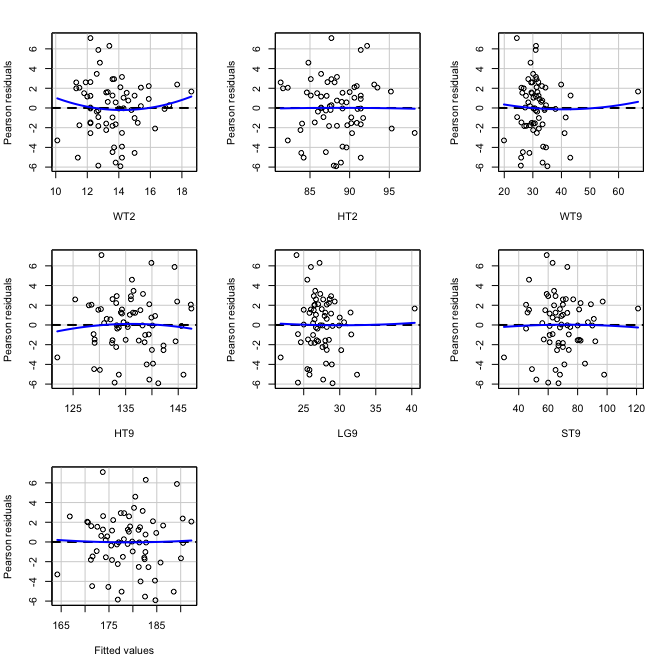
\includegraphics[width = \textwidth]{ResidualPlotsModel.png}
    \end{center}
  \end{figure}
  \begin{figure}[H]
    \begin{center}
    \caption{Residual Plot for Standard Model}
    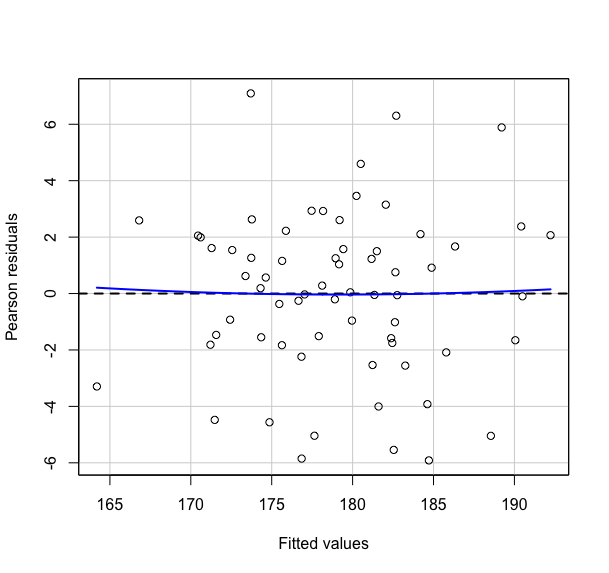
\includegraphics[width = \textwidth]{ResidualPlotModel.png}
    \end{center}
  \end{figure}
  \begin{figure}[H]
    \begin{center}
    \caption{Residual Plot Cooks Distance}
    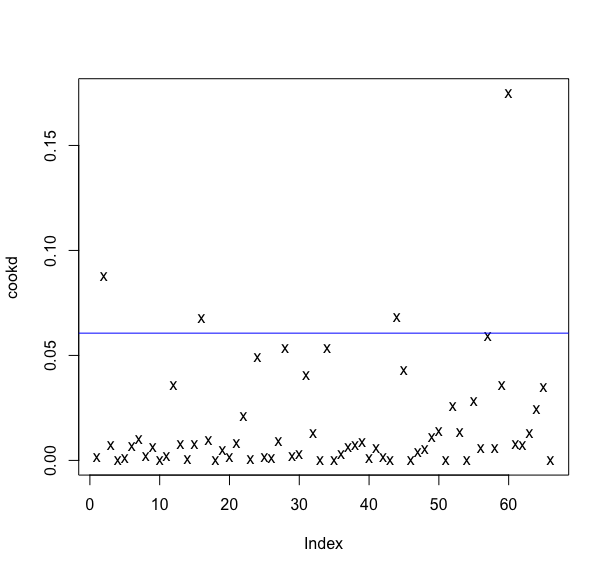
\includegraphics[width = \textwidth]{CooksDModel.png}
    \end{center}
  \end{figure}
  Predictor transformed model.\\
  \textbf{Code:}
  \begin{center}
  \lstinputlisting{r11.txt}
  \end{center} 
  \begin{figure}[H]
    \begin{center}
    \caption{Predictor Residual Plots for Standard Model}
    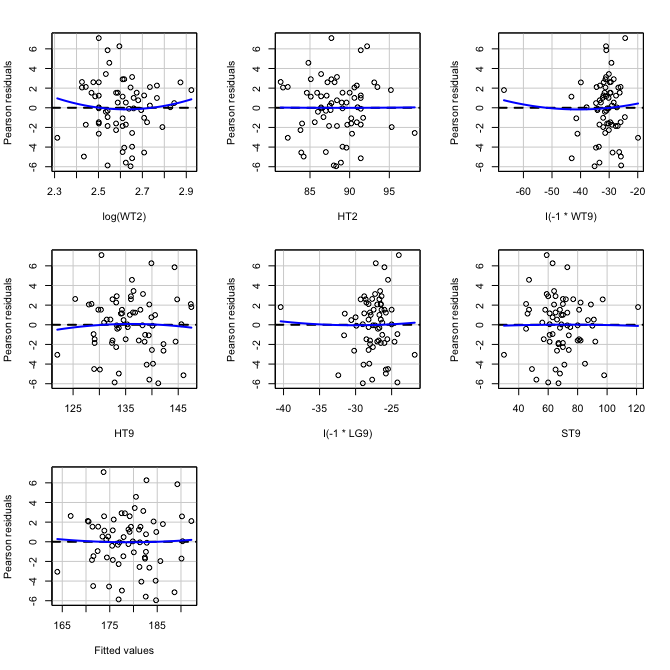
\includegraphics[width = \textwidth]{ResidualsPredTransformed.png}
    \end{center}
  \end{figure}
  \begin{figure}[H]
    \begin{center}
    \caption{Residual Plot for Standard Model}
    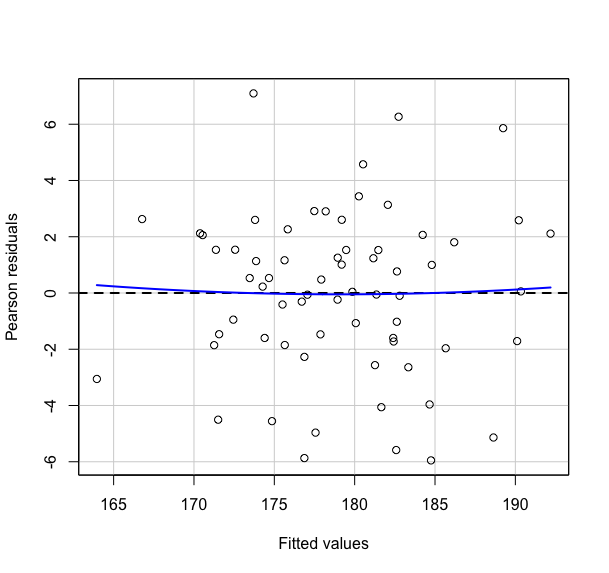
\includegraphics[width = \textwidth]{ResidualPlotPredTrans.png}
    \end{center}
  \end{figure}
  \begin{figure}[H]
    \begin{center}
    \caption{Residual Plot Cooks Distance}
    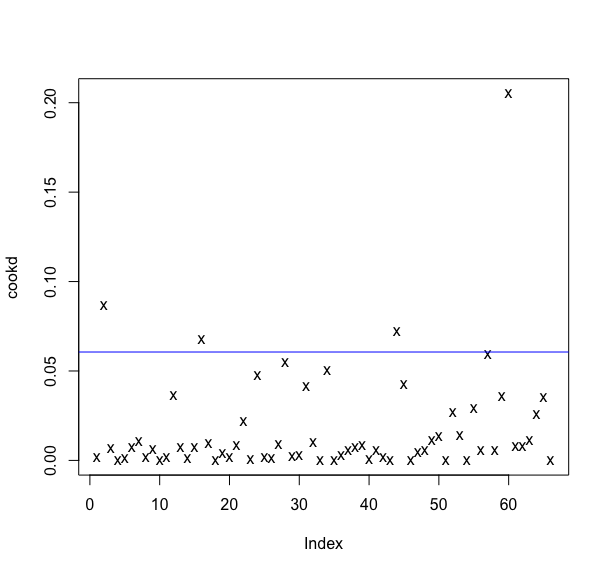
\includegraphics[width = \textwidth]{InfluencePredTrans.png}
    \end{center}
  \end{figure}
  As we can see the diagnostic scored almost exactly the same, and comparing model summary reports they are also very similar.
  It seems as though there is no significant gain in transforming this data. I would likely use the plain data.   
\end{exercise}
\newpage


\begin{exercise}{4.6} In the simple linear regression of log(fertility) on pctUrban using UN11 data the fitted model is, 
  \begin{equation*}
    log(fertility) = 1.501 - 0.01pctUrban
  \end{equation*}
  Provide an interpretation of the estimated coefficient for pct Urban. \\
  \solution  For every one unit increase of pctUrban we can expect the mean response of fertility to decrease by a factor of
  $e^{.01} \approx 1.01$ or approximately 1 percent. 
  \end{exercise}




\end{document}





















